% Modules generaux
\documentclass[11pt]{article}
\usepackage[utf8]{inputenc}
\usepackage[T1]{fontenc}
\usepackage[francais]{babel} % prise en charge du francais
\usepackage[table]{xcolor} % tableaux
\usepackage{longtable}
\usepackage{booktabs}
\usepackage{graphicx} % images
\usepackage{framed}
\usepackage{float}
\usepackage[font=small]{caption}

% Marges
\usepackage[left=2cm,right=2cm,top=2cm,bottom=2cm]{geometry}

% Personnalisation des titres
\usepackage{titlesec}
\titlespacing{\section}{0em}{4em}{1em}
\titlespacing{\subsection}{0em}{2em}{0em}
\titlespacing{\subsubsection}{0em}{0.5em}{0em}

% Mise en page
\setlength{\parskip}{1.2em}
\renewcommand{\floatpagefraction}{1}

% Couleurs personnalisées
\usepackage{color}
\definecolor{lightgray}{gray}{0.98}
\definecolor{gray}{rgb}{0.6, 0.6, 0.65}
\definecolor{green}{rgb}{0.133, 0.545, 0.133}
\definecolor{blue}{rgb}{0, 0, 1}
\definecolor{red}{rgb}{0.6, 0.1, 0.1}

% Liens hypertextes
\usepackage{hyperref}
\hypersetup{
	colorlinks=true,
	breaklinks=true,
	urlcolor=blue,
	linkcolor=blue,
	pdfborder=000,
	pdftex=true
}

% Mise en forme des codes python
\usepackage{listingsutf8}
\lstset{
	language=python,
	inputencoding=utf8/latin1,
	extendedchars=true,
	keywordstyle=\bfseries\ttfamily\color{blue},
	identifierstyle=\ttfamily,
	commentstyle=\color{gray},
	stringstyle=\ttfamily\color{green},
	showstringspaces=false,
	basicstyle=\footnotesize\ttfamily,
	tabsize=2,
	breaklines=true,
	extendedchars=true,
	xleftmargin=1cm,
	xrightmargin=1cm,
	backgroundcolor=\color{lightgray},
	literate=%
		{é}{{\'{e}}}1
		{è}{{\`{e}}}1
		{ê}{{\^{e}}}1
		{ë}{{\¨{e}}}1
		{û}{{\^{u}}}1
		{ù}{{\`{u}}}1
		{â}{{\^{a}}}1
		{à}{{\`{a}}}1
		{î}{{\^{i}}}1
		{ô}{{\^{o}}}1
		{ç}{{\c{c}}}1
}
\newcommand{\passthrough}[1]{#1}

% Commandes personnalisées
\newcommand{\bslash}{\texttt{\symbol{92}}}

\newcommand{\reponse}{\begin{tabbing}
\hspace{2cm}\=\kill
Réponse \> ............................................................................................ \\
 \> ............................................................................................
\end{tabbing}
}
\newenvironment{note}{%
	\begin{tabular}[t t]{c c}
		
\includegraphics{img/tips.png} &
		\begin{minipage}[c]{0.9\linewidth}
}{%
		\end{minipage}
	\end{tabular}
}

\newsavebox{\mybox}
\newenvironment{objectifs}{
	\begin{lrbox}{\mybox}
		\begin{minipage}{0.9\textwidth}
			\vspace{1em}
			\begin{tabular}[t t]{c c}
				
\includegraphics[width=0.1\linewidth]{img/goals.jpg} &
				\begin{minipage}[c]{0.8\linewidth}
					\hspace{2em}\textbf{\large{Objectifs :}} \\
}{
				\end{minipage}
			\end{tabular}
			\vspace{1em}
		\end{minipage}
	\end{lrbox}
	\fbox{\usebox{\mybox}}
}

\newcommand{\code}[1]{\lstinline{#1}}

\newenvironment{python}{%
	\begin{lstlisting}
}{%
	\end{lstlisting}
}

\renewenvironment{quote}{\begin{framed}}{\end{framed}}

% Patch : probleme avec les tightlist
\def\tightlist{}

% Patch : probleme avec les images
\let\origfigure=\figure
\let\endorigfigure=\endfigure
\renewenvironment{figure}[1][]{%
  \origfigure[H]
}{%
  \endorigfigure
}

% Patch : probleme de taille maximale des images
\makeatletter
\def\maxwidth{\ifdim \Gin@nat@width > 0.8\linewidth 0.8\linewidth \else \Gin@nat@width \fi}
\makeatother
\let\oldincludegraphics\includegraphics
\renewcommand{\includegraphics}[1]{\oldincludegraphics[width=\maxwidth]{#1}}


%%%%%%%%%%%%%%%%%%%%%%%%%%%%%%%%%%%%%%%%
% Informations générales sur le document
%%%%%%%%%%%%%%%%%%%%%%%%%%%%%%%%%%%%%%%%
\title{Utilisation de données vecteur avec Python}
\author{Clément Delgrange}
\date{Mars 2018}

% Définition des entêtes et pieds de page
\usepackage{fancyhdr}
\pagestyle{fancy}
\fancyhf{}
\renewcommand{\headrulewidth}{0pt}
\fancyfoot[L]{Clément Delgrange}
\fancyfoot[C]{-\thepage-}
\fancyfoot[R]{Utilisation de données vecteur avec Python}
\renewcommand{\footrulewidth}{0.5pt}


%%%%%%%%%%%%%
% Le document
%%%%%%%%%%%%%
\begin{document}

\begin{titlepage}
	\begin{sffamily}
		\begin{flushleft}
			% 
\includegraphics{img/logos/ign-logo-ensg.jpg}\\[1.5cm]
		\end{flushleft}
		\begin{flushright}
			% pour mettre une image en haut à droite
		\end{flushright}

		\vspace{4cm}

		\begin{center}
			\hrule
				\vspace{1em}
				{\small \textit{Programmation SIG}}\\
				\vspace{0.5cm}
				{\huge \bfseries Utilisation de données vecteur avec Python}
				\vspace{1cm}
			\hrule

			\vspace{3.5cm}
			%\includegraphics[width=400px]{images/logo_python.png}
			\vspace{5cm}

			\large \textit{Clément Delgrange}\\
			\small \textit{Mars 2018}
		\end{center}
	\end{sffamily}
\end{titlepage}


\addtocontents{toc}{
	\protect\setlength{\parskip}{0pt}
}
\setcounter{tocdepth}{2}
\renewcommand{\partname}{Partie}
\tableofcontents
\newpage

\begin{objectifs}
Connaître les différentes primitives géométriques

Manipuler des objets géolocalisés et effectuer quelques opérations spatiales

Ouvrir des fichiers géographiques de différents formats, dans différentes projections

Visualiser les données géolocalisées, créer des cartes statiques et interactives
\end{objectifs}

\hypertarget{introduction}{%
\section{Introduction}\label{introduction}}

La première partie du cours nous a permis d'établir un panorama des
possibilités offertes par l'ensemble des techniques de programmation
SIG. Dans ce chapitre nous nous proposons d'aborder la programmation SIG
en laissant le SIG bureautique traditionnel de côté. Au lieu de cela,
nous préférons nous concentrer sur la base de notre métier : la donnée
géographique. Nous commencerons ainsi par un bref rappel des modes de
représentation de l'information géographique. Puis nous verrons comment
le langage de programmation Python nous permet de manipuler cette
information géographique : manipulation de géométries vecteur,
opérations spatiales, gestion des projections, représentation, etc. Nous
nous situerons donc ici plutôt dans la dernière des catégories de
développements SIG que nous avons établit dans la première partie de ce
cours, les applications autonomes, même si les techniques apprises ici
pourrons nous être utiles pour développer, par exemple, des plugins pour
un SIG.

\hypertarget{le-choix-de-python-comme-langage-de-programmation}{%
\subsection{Le choix de Python comme langage de
programmation}\label{le-choix-de-python-comme-langage-de-programmation}}

Dans cette partie, comme dans beaucoup de suivantes, nous utiliserons
exclusivement le langage de programmation Python. Aujourd'hui Python est
probablement le langage de programmation le plus utilisé en géomatique.
L'écosystème Python s'est enrichi ses dernières années de nombreuses
libraires à visées géospatiales. C'est aussi le langage que les SIG ont
choisi depuis plusieurs années pour exécuter des scripts de
géotraitements (ArcGIS, QGIS, etc.). Nous pouvons évoquer plusieurs
raisons à cela:

\begin{itemize}
\tightlist
\item
  sa facilité d'utilisation et d'apprentissage pour des ``non
  informaticiens'';
\item
  il est gratuit et open-source;
\item
  il est assez facilement intégrable à d'autres langages
  (\passthrough{\lstinline!C!}, \passthrough{\lstinline!C++!});
\item
  de nombreuses libraires de calculs numériques existent
  (\passthrough{\lstinline!numpy!}, \passthrough{\lstinline!scipy!},
  \passthrough{\lstinline!pandas!}, etc.);
\item
  les libraires fondamentales de la géomatique
  (\passthrough{\lstinline!PROJ.4!}, \passthrough{\lstinline!GDAL!},
  etc.) bénéficient de bindings Python.
\end{itemize}

\hypertarget{repruxe9sentation-de-linformation-guxe9ographique}{%
\section{Représentation de l'information
géographique}\label{repruxe9sentation-de-linformation-guxe9ographique}}

\hypertarget{raster-vs.vecteur}{%
\subsection{Raster vs.~vecteur}\label{raster-vs.vecteur}}

Deux façons de stocker les données géolocalisées : le mode vecteur et le
mode raster. Ces deux modes permettent de représenter la même
information mais le font de manière différente.

En mode raster, le monde réel est représenté sous la forme de matrice où
chaque case prend une valeur reflétant la valeur de l'information à
représenter. Des matrices multi-dimensionnelles (ie. à plusieurs bandes)
sont fréquemment utilisées pour représenter les phénomènes complexes.

\begin{figure}
\centering

\includegraphics{img/cours1/representation_vecteur.png}
\caption{Représentation vecteur}
\end{figure}

Le mode vecteur représente l'information géographique sous forme de
géométries.

\begin{figure}
\centering
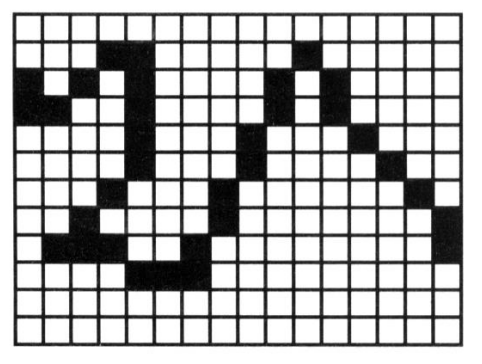
\includegraphics{img/cours1/representation_raster.png}
\caption{Représentation raster}
\end{figure}

Les géométries peuvent être dotées d'un sémantique (ie. des attributs)
et liées entre elles grâce à des liens de topologies (ex : deux routes
données sont connectées en un carrefour, ne sont pas connectées, se
croisent à un pont mais ne sont pas connectées, etc.).

Si les rasters sont plus faciles à créer, l'analyse des données vecteur
est plus aisée. Dans la suite de cette partie nous nous focaliserons sur
les données vecteur, tandis que la prochaine partie reviendra sur les
données raster.

\hypertarget{les-primitives-guxe9omuxe9triques}{%
\subsection{Les primitives
géométriques}\label{les-primitives-guxe9omuxe9triques}}

Dans le mode vecteur le monde réel est donc représenté à l'aide de
géométries. Dans sa norme \emph{Simple Feature Access}\footnote{\url{http://www.opengeospatial.org/standards/sfa}},
l'Open Geospatial Consortium (OGC) définit huit primitives géométriques
:

\begin{figure}
\centering
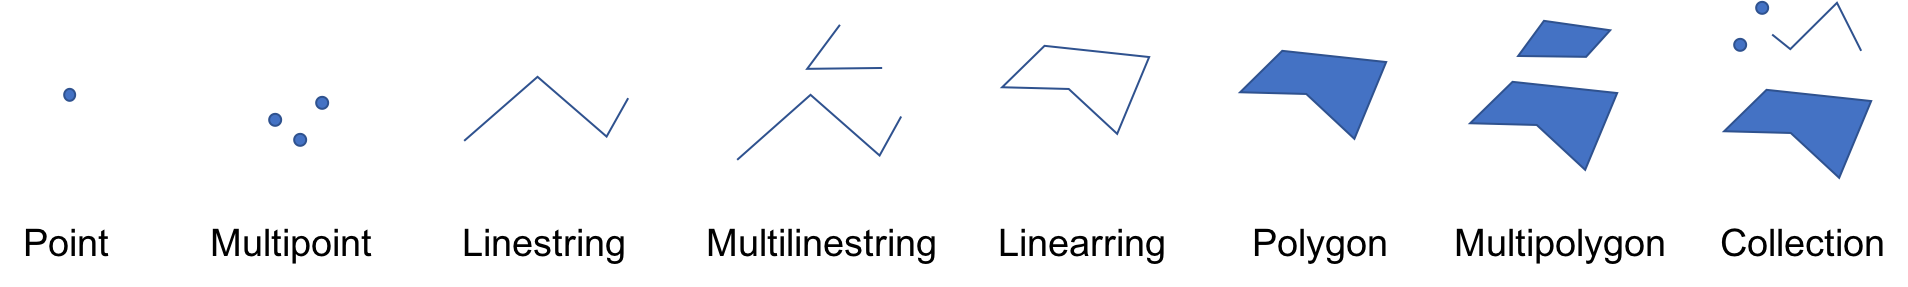
\includegraphics{img/cours1/primitives_geometriques.png}
\caption{Les primitives géométriques}
\end{figure}

\begin{note}
"L'Open Geospatial Consortium, ou OGC, est un consortium international pour développer et promouvoir des standards ouverts, les spécifications OpenGIS, afin de garantir l'interopérabilité des contenus, des services et des échanges dans les domaines de la géomatique et de l'information géographique." (source Wikipedia)

Les principaux acteurs du marché (Esri, Oracle, etc.) ainsi que des instituts nationaux sont membre de l'OGC.
Aussi il est fort probable qu'une norme publiée par l'OGC soit aussitôt reprise par l'ensemble de la communauté géomatique.
\end{note}

Le modèle géométrique complet vous est donné ci-dessous. Il nous
intéresse pour comprendre comment sont structurées les données
géographiques vecteur. Vous constaterez, qu'en plus des huit primitives
géométriques, d'autres classes abstraites sont introduites pour donner
du sens au modèle et lier les primitives géométriques entre elles.

\begin{figure}
\centering
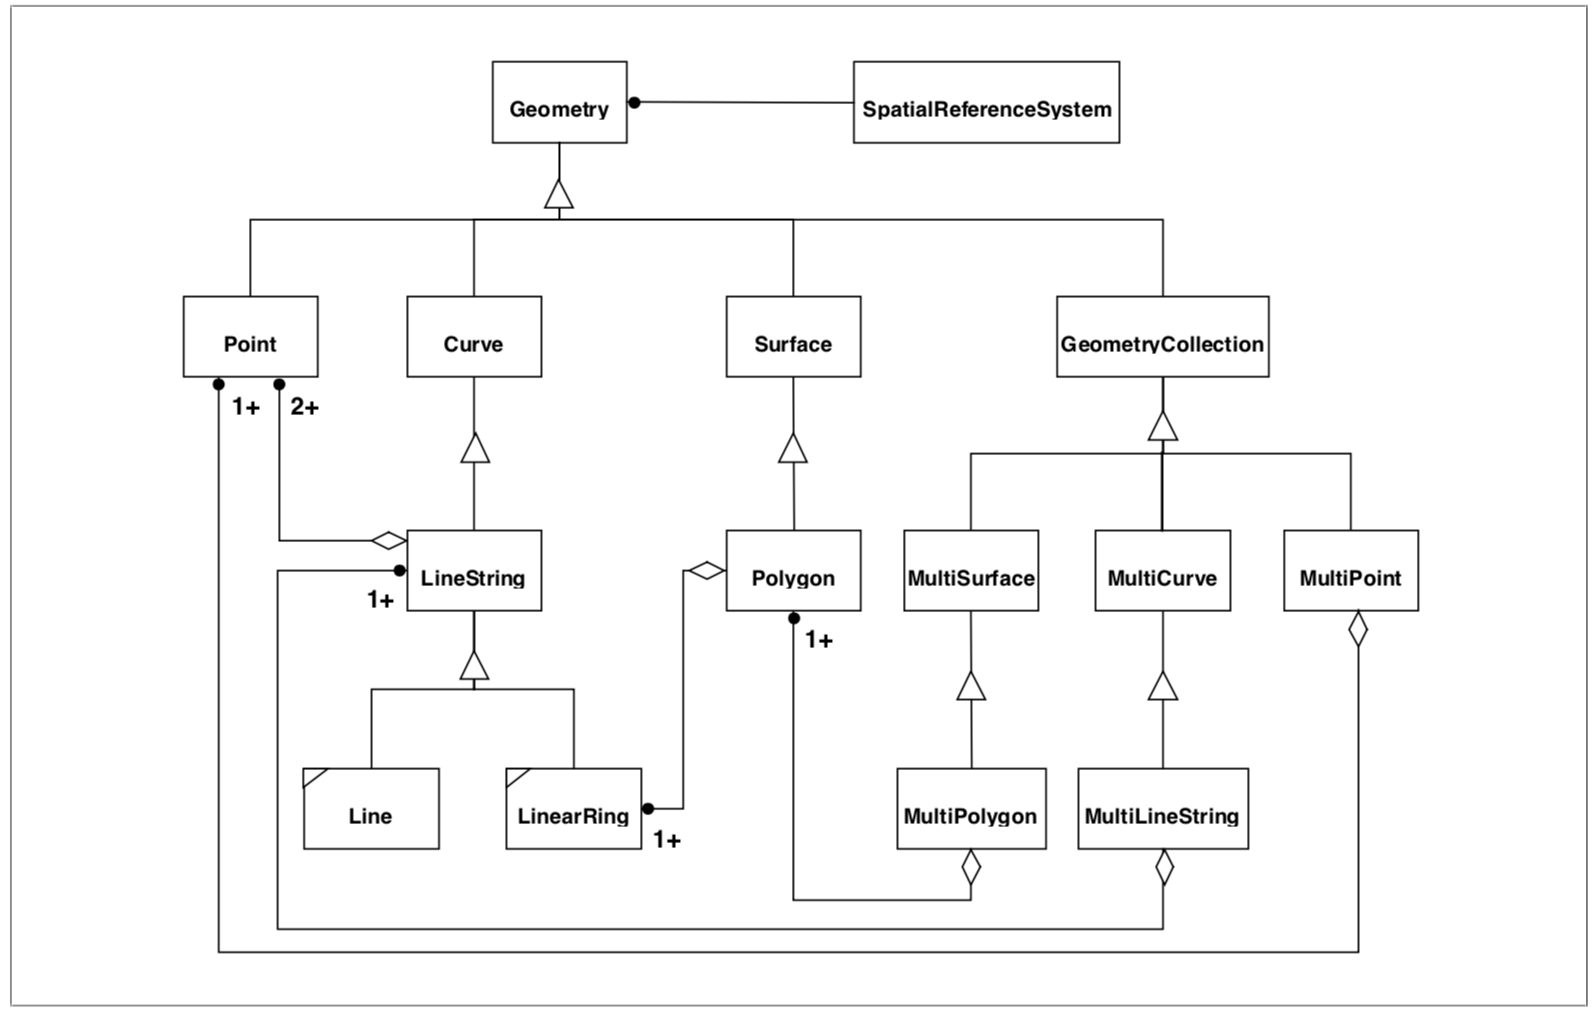
\includegraphics{img/cours1/modele_geometrique.png}
\caption{Hiérarchie des classes géométriques}
\end{figure}

Ce modèle nous intéresse également parce qu'il est repris dans la
plupart des outils que nous utiliserons. C'est notamment le cas de la
librairie GEOS maintenue par la Fondation Open Source Geospatial (OSGeo)
qui occupe une place centrale dans le monde de la géomatique. Basée sur
la Java Topology Suite (JTS)\footnote{\url{https://github.com/locationtech/jts}},
cette librairies est notamment utilisée dans PostGIS ou
\passthrough{\lstinline!shapely!} que nous utiliserons dans la suite de
ce chapitre.

\begin{note}
"La Fondation Open Source Geospatial (OSGeo) est une organisation non gouvernementale fondée en 2006 pour soutenir et construire une offre de logiciels open source en géomatique." (source Wikipedia)

Alors que l'OGC édite des normes favorisant l'interopérabilité et les échanges de données, l'OSGeo soutient le développement d'outils open source mettant en oeuvre ces normes.
\end{note}

\hypertarget{validituxe9-des-guxe9omuxe9tries}{%
\subsection{Validité des
géométries}\label{validituxe9-des-guxe9omuxe9tries}}

Au delà d'une simple hiérarchie entre les objets géométriques, la norme
\emph{Simple Feature Access} définie également des règles de validité
pour chacune des géométries.

Ci dessous nous présentons quelques exemples de polygones invalides. Des
règles similaires existent pour les autres types de géométries (lignes
auto-intersectées, etc.).

\begin{figure}
\centering
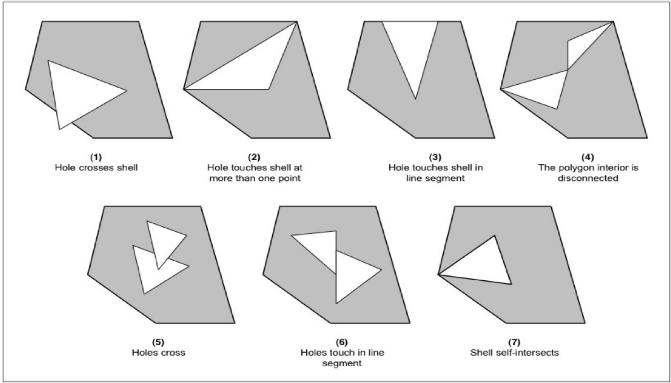
\includegraphics{img/cours1/validite_geometries.png}
\caption{Exemples de polygones invalides (source site web de JTS)}
\end{figure}

\hypertarget{les-opuxe9rations-spatiales}{%
\subsection{Les opérations
spatiales}\label{les-opuxe9rations-spatiales}}

Enfin, la norme \emph{Simple Feature Access} définit les opérations
spatiales permises pour chaque type de géométrie. Ce sont les opérations
spatiales que l'on retrouve dans les outils SIG communs :

\begin{itemize}
\tightlist
\item
  buffer, rectangle englobant, enveloppe convexe, etc. pour les
  opérations n'impliquant qu'une seule géométrie;
\item
  intersections, union, différence, différence symétrique, etc. pour les
  opérations impliquant plusieurs géométries.
\end{itemize}

\hypertarget{la-librairie-shapely}{%
\subsection{\texorpdfstring{La librairie
\texttt{shapely}}{La librairie shapely}}\label{la-librairie-shapely}}

Le module \passthrough{\lstinline!shapely!} a été créé par Sean Gillies
pour permettre d'effectuer, avec un syntaxe \emph{pythonique}, ce qu'il
est possible de faire avec GEOS pour manipuler et analyser des
géométries. Aussi tout comme GEOS, \passthrough{\lstinline!shapely!}
reprend une bonne part des principes exposés dans la norme \emph{Simple
Feature Access} de l'OGC.

\passthrough{\lstinline!shapely!} ne traite que des géométries et ne
s'intéresse pas aux formats de données (lecture/écriture de fichiers) ou
encore aux reprojections. Il s'agit d'un parti pris de Sean Gillies qui
a par ailleurs travaillé sur d'autres librairies pour ces taches : par
exemple \passthrough{\lstinline!fiona!} pour la lecture/écriture de
shapefiles ou \passthrough{\lstinline!affine!} pour effectuer des
transformations affines.

Les notions d'\emph{intérieur} (interior), de \emph{frontière}
(boundary) et d'\emph{extérieur} (exterior) sont introduites par la
librairie. L'union de ces trois ensemble correspond à l'ensemble du
plan.

\begin{itemize}
\tightlist
\item
  l'intérieur d'un point est égale au point lui même, sa frontière est
  nulle et l'extérieur correspond à tous les autres points;
\item
  pour une ligne (linestring ou linearring), l'intérieur équivaut à
  l'ensemble des points sur sa longueur, la frontière aux deux
  extrémités et l'extérieur au reste des points;
\item
  pour un polygone, l'intérieur est composé des points à l'intérieur de
  celui-ci, la frontière à une ou plusieurs lignes constituant le
  contour du polygone et l'extérieur au reste des points (y compris ceux
  à l'intérieur des trous).
\end{itemize}

\begin{figure}
\centering
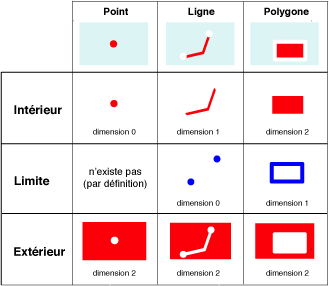
\includegraphics{img/cours1/shapely_interieur_exterieur.png}
\caption{Notions d'intérieur et d'extérieur dans shapely}
\end{figure}

La syntaxe pour créer des géométries avec
\passthrough{\lstinline!shapely!} est la suivante :

\begin{lstlisting}
>>> from shapely.geometry import Point,
>>> pt = Point([2, 3])
>>> ls = LineString([[0, 0], [1, 1], [2, 0]])
>>> poly = Polygon([[0, 0], [1, 1], [2, 0], [0, 0]])
\end{lstlisting}

Une fois la géométrie définie, il est ensuite possible d'accéder à
certaines propriétés :

\begin{lstlisting}
>>> ls.bounds  # rectangle englobant de la ligne
(0.0, 0.0, 2.0, 1.0)
>>> poly.area  # aire du polygone
1.0
>>> poly.exterior  # linearring constituant le contour extérieur
<shapely.geometry.polygon.LinearRing at 0x107d3d6a0>
\end{lstlisting}

Les coordonnées d'un objet s'obtiennent à l'aide de la propriété
\passthrough{\lstinline!coords!} qui renvoie un objet de type
\passthrough{\lstinline!CoordinateSequence!}. Pour pouvoir afficher les
coordonnées, on peut le transformer en liste :

\begin{lstlisting}
>>> ls.coords  # objet CoordinateSequence de la linestring
<shapely.coords.CoordinateSequence at 0x107d3d278>
>>> list(ls.coords)
[(0.0, 0.0), (1.0, 1.0), (2.0, 0.0)]
>>> list(poly.exterior.coords)
[(0.0, 0.0), (1.0, 1.0), (2.0, 0.0), (0.0, 0.0)]
\end{lstlisting}

Il est aussi possible d'effectuer des opérations géométriques :

\begin{lstlisting}
buff = pt.buffer(2)  # retourne le polygone construit en effectuant un buffer de 2 autour du point
\end{lstlisting}

La documentation complète de la librairie se trouve à l'adresse suivante
: \url{https://shapely.readthedocs.io}.

\hypertarget{exercices}{%
\subsection{Exercices}\label{exercices}}

\begin{enumerate}
\def\labelenumi{\arabic{enumi}.}
\tightlist
\item
  Ecrire une fonction prenant une liste de point
  \passthrough{\lstinline!shapely!} et retournant deux éléments :
\end{enumerate}

\begin{itemize}
\tightlist
\item
  un booléan indiquant si le polygone \passthrough{\lstinline!shapely!}
  dont le contour extérieur est constitué de la suite de points est
  valide;
\item
  une chaîne de caractère détaillant le motif d'invalidité (ou une
  chaîne vide s'il est valide).
\end{itemize}

\begin{enumerate}
\def\labelenumi{\arabic{enumi}.}
\setcounter{enumi}{1}
\tightlist
\item
  Ecrire une fonction qui prend en entrée deux linestrings et retourne
  leur intersection. Le deux linestring et l'intersection seront ensuite
  dessinées dans un graphique matplotlib.
\item
  Ecrire un programme qui prend en entrée un fichier csv\footnote{Comma-separated
    Values (CSV) : format représentant des données tabulaires sous forme
    de de valeurs séparées par des virgules.} contenant les coordonnées
  d'une liste de points et une distance
  \passthrough{\lstinline!dist\_ref!} et qui retourne un booléen
  indiquant si un point se situe à une distance supérieure à
  \passthrough{\lstinline!dist\_ref!} de tous les autres points ou si
  chacun des points se situe à moins de
  \passthrough{\lstinline!dist\_ref!} d'un autre point.
\end{enumerate}

\hypertarget{indices}{%
\subsubsection{Indices}\label{indices}}

\begin{enumerate}
\def\labelenumi{\arabic{enumi}.}
\tightlist
\item
  L'essentiel de la documentation de \passthrough{\lstinline!shapely!}
  peut se retrouver sur une seule page web à l'adresse :
  \url{https://shapely.readthedocs.io/en/latest/manual.html}. Essayer
  d'y effectuer une recherche avec un mot clé adéquat (en anglais ;-)).
\item
  Les instructions suivantes permettent d'afficher un point puis une
  ligne dans un graphique matplotlib :
\end{enumerate}

\begin{lstlisting}
import matplotlib.pyplot as plt

plt.plot(2, 3)  # dessine le point (2, 3)
plt.plot([0, 1, 2], [0, 1, 0])  # dessine la ligne [(0, 0), (1, 1), (2, 0)]
plt.show()
\end{lstlisting}

Vous pouvez consulter la documentation de la fonction
\passthrough{\lstinline!plot!} pour avoir plus d'options d'affichage
(couleurs, formes, etc.) :
\url{https://matplotlib.org/api/pyplot_api.html\#matplotlib.pyplot.plot}.
3. Un ficheir csv est un fichier texte. Vous pouvez le lire comme un
fichier texte classique ou utiliser une librairie adaptée.

\hypertarget{les-formats-duxe9change}{%
\section{Les formats d'échange}\label{les-formats-duxe9change}}

Depuis une trentaine d'années, les SIG se sont implantés dans de
nombreux domaines. Diverses solutions commerciales se sont développées
permettant à l'utilisateur un vaste choix parmi ces solutions. Cette
diversité de solutions implique une diversité de formats, chaque éditeur
de logiciel étant à l'origine de sont propre format.

Lorsque les utilisateurs cherchent à faire communiquer leurs
applications, ils sont confrontés au problème de
l'\emph{interopérabilité} : la capacité des système à s'échanger et se
partager des données.

Dans ce contexte nous distinguerons les formats dits \emph{ouverts}
(pensons aux shapefiles d'Esri) de ceux dits \emph{fermés} (les
géodatabases d'Esri). Par ouverts/fermés nous entendons que les
spécifications de ces formats sont respectivement publiques ou pas.
Naturellement des formats ouverts permettent l'interopérabilité des
données tandis que les formats fermés la limite en imposant
l'utilisation d'un logiciel particulier.

La problématique sera identique pour le développeur : un format ouvert
sera manipulable au travers de différentes librairies. Les formats
fermés ne le seront généralement que via les librairies de l'éditeur de
SIG propriétaire du format.

Aujourd'hui les données ont de plus en plus besoin d'être échangées
entre divers acteurs. On comprendra alors aisément que l'importance des
formats ouverts dans ce contexte.

Pour les données vecteur, l'OGC a mis en avant le \emph{well-known text}
(WKT) dans la norme \emph{Simple Feature Access} pour décrire de manière
textuelle tous les types de géométrie. D'autres formats permettant
d'inclure des informations sémantiques sur les géométries ont également
été mis en oeuvre par la communauté : le GeoJSON, le GML, etc. Parmi eux
le \textbf{GeoJSON} semble aujourd'hui être plébiscité par la communauté
SIG pour manipuler les données vecteur.

\hypertarget{le-geojson}{%
\subsection{Le GeoJSON}\label{le-geojson}}

Basé sur le format JSON (JavaScript Open Notation), le GeoJSON permet de
représenter toutes les primitives géométriques définies par l'OGC. Il
est lisible par un humain et manipulable par la plupart des libraires
géospatiales ainsi que par les principaux SIG du marché.

\begin{note}
Le format JSON (JavaScript Open Notation) est un format textuel qui permet de représenter une information structurée.
Il est fréquemment utilisé comme format d'échange dans le monde du web en raison de sa facilité de mise en oeuvre.
Un document JSON ne comporte que deux types d'éléments : des couples clé/valeur et des listes ordonnées de valeurs.
Les types permis pour les valeurs sont : nombres, chaînes de caractères, booléens, null, liste ordonnées ou objet JSON.
\end{note}

La structure du GeoJSON est celle d'un dictionnaire en Python. Les
différents types de géométries sont listés dans le tableau suivant :

\begin{tabular}{|c|l|}
    \hline
    Point &
    \begin{lstlisting}
{ "type": "Point",
    "coordinates": [30, 10]
}
    \end{lstlisting} \\
    \hline
    Polyligne &
    \begin{lstlisting}
{ "type": "LineString",
    "coordinates": [
        [30, 10], [10, 30], [40, 40]
    ]
}
    \end{lstlisting} \\
    \hline
    \begin{tabular}{c}
        Polygone \\
        (y compris avec trous)
    \end{tabular} &
    \begin{lstlisting}
{ "type": "Polygon",
    "coordinates": [
        [[35, 10], [45, 45], [15, 40], [10, 20], [35, 10]],
        [[20, 30], [35, 35], [30, 20], [20, 30]]
    ]
}
    \end{lstlisting} \\
    \hline
    Multi-point &
    \begin{lstlisting}
{ "type": "MultiPoint",
    "coordinates": [
        [10, 40], [40, 30], [20, 20], [30, 10]
    ]
}
    \end{lstlisting} \\
    \hline
    Multi-polyligne &
    \begin{lstlisting}
{ "type": "MultiLineString",
    "coordinates": [
        [[10, 10], [20, 20], [10, 40]],
        [[40, 40], [30, 30], [40, 20], [30, 10]]
    ]
}
    \end{lstlisting} \\
    \hline
    Multi-polygone &
    \begin{lstlisting}
{ "type": "MultiPolygon",
    "coordinates": [
        [
            [[40, 40], [20, 45], [45, 30], [40, 40]]
        ],
        [
            [[10, 30], [10, 10], [40, 5], [40, 30], [20, 35]],
            [[30, 20], [20, 15], [20, 25], [30, 20]]
        ]
    ]
}
    \end{lstlisting} \\
    \hline
\end{tabular}

Une entité géométrique \passthrough{\lstinline!Feature!} possède une
balise \passthrough{\lstinline!geometry!} et une balise
\passthrough{\lstinline!properties!} pour la sémantique de la géométrie:

\begin{lstlisting}
{
  "type": "Feature",
  "geometry": {
    "type": "Polygon",
    "coordinates": [
      [
        [100.0, 0.0],
        [101.0, 0.0],
        [101.0, 1.0],
        [100.0, 1.0],
        [100.0, 0.0]
      ]
    ]
  },
  "properties": {
    "nom": "Paris",
    "population": 2000000
  }
}
\end{lstlisting}

Le type \passthrough{\lstinline!FeatureCollection!} permet de regrouper
un ensemble de géométries de types différents au sein d'une même entité
géométrique :

\begin{lstlisting}
{ "type": "FeatureCollection",
    "features": [
      { "type": "Feature",
        "geometry": {
          "type": "Point",
          "coordinates": [...]
        },
        "properties": {
          "prop0": "value0"
        }
      },
      { "type": "Feature",
        "geometry": {
          "type": "LineString",
          "coordinates": [...]
        },
        "properties": {
          "prop0": "value0",
          "prop1": 0.0
        }
      },
      { "type": "Feature",
         "geometry": {
           "type": "Polygon",
           "coordinates": [...]
         },
         "properties": {
           "prop0": "value0",
           "prop1": 123456
           }
         }
       ]
     }
\end{lstlisting}

\hypertarget{le-protocole-__geo_interface__}{%
\subsection{\texorpdfstring{Le protocole
\texttt{\_\_geo\_interface\_\_}}{Le protocole \_\_geo\_interface\_\_}}\label{le-protocole-__geo_interface__}}

Sean Gillies a proposé un protocole pour représenter les informations
géographiques vecteur dans Python en se basant sur le GeoJSON :
\url{https://gist.github.com/sgillies/2217756} Ce protocole est adopté
petit à petit par la communauté Python géomatique et les les principales
libraires l'implémentent maintenant (\passthrough{\lstinline!shapely!},
\passthrough{\lstinline!arcpy!}, \passthrough{\lstinline!geojson!},
\passthrough{\lstinline!PySAL!}, etc.).

Par exemple avec \passthrough{\lstinline!shapely!}, les instructions
suivantes retournent la représentation GeoJSON d'un multipoint :

\begin{lstlisting}
>>> from shapely.geometry import MultiPoint
>>> mpt = MultiPoint([[0, 0], [1, 0], [0, 1], [1, 1]])
>>> mpt.__geo_interface__
{'coordinates': ((0.0, 0.0), (1.0, 0.0), (0.0, 1.0), (1.0, 1.0)),
 'type': 'MultiPoint'}
\end{lstlisting}

\hypertarget{les-fichiers-de-formes}{%
\subsection{Les fichiers de formes}\label{les-fichiers-de-formes}}

Le format shapefile, ou \emph{fichier de formes}, a initialement été
développé par Esri pour ses logiciels SIG. Aujourd'hui les
spécifications de ce format ont été rendues publiques, ce qui lui a
permis petit à petit de s'imposer comme un standard. Il est lisible dans
la majorité des logiciels du marché de la géomatique : ArcGIS, QGIS,
Autodesk Map, Grass, GvGIS, MapServer, etc.

Un fichier de forme est toujours composé de plusieurs fichiers portant
nécessairement le même nom :

\begin{itemize}
\tightlist
\item
  le \passthrough{\lstinline!.shp!} contenant les géométries;
\item
  le \passthrough{\lstinline!.dbf!} stockant les informations
  sémantiques relatives aux géométries;
\item
  le \passthrough{\lstinline!.shx!} qui stocke un index des géométries.
\end{itemize}

D'autres fichiers annexes peuvent être présents. Citons notamment :

\begin{itemize}
\tightlist
\item
  un index spatial (\passthrough{\lstinline!.sbx!});
\item
  la définition du système de coordonnées utilisé
  (\passthrough{\lstinline!.prj!}).
\end{itemize}

Pour ouvrir un fichier de formes en Python, nous pouvons utiliser la
librairie \passthrough{\lstinline!fiona!}
(\url{https://toblerity.org/fiona/}).

La syntaxe pour ouvrir un fichier est semblable à celle d'ouverture d'un
fichier ``classique'', à ceci près que l'itération sur le contenu du
fichier ouvert retourne la
\passthrough{\lstinline!\_\_geo\_interface\_\_!} des géométries du
shapefile :

\begin{lstlisting}
>>> import fiona
>>> with fiona.open('test.shp', 'r') as shp_file:
...     for geom in shp_file:
...         print(geom)
...
{'coordinates': (0.0, 0.0), 'type': 'Point'}
{'coordinates': (2.0, 0.4), 'type': 'Point'}
{'coordinates': (4.0, 2.0), 'type': 'Point'}
\end{lstlisting}

\hypertarget{exercices-1}{%
\subsection{Exercices}\label{exercices-1}}

Le format gpx est un format d'échange de données GPS, notamment utilisé
par les montres GPS de sport\footnote{Norme GPX :
  \url{http://www.topografix.com/GPX/1/1/}}. Il est basé sur le langage
de balise XML.

Créer une fonction prenant en entrée un fichier gpx et retournant une
géométrie shapely représentant la trace contenue dans le fichier. Tester
votre fonction avec le fichier \passthrough{\lstinline!trace.gpx!}.

Ecrire ensuite une seconde fonction permettant d'écrire un fichier
GeoJSON à partir de la géométrie shapely précédente.

\hypertarget{indices-1}{%
\subsubsection{Indices}\label{indices-1}}

Pour lire le fichier gpx, plusieurs possibilités sont envisageables :

\begin{itemize}
\tightlist
\item
  lire le fichier comme un ficher texte et analyser son contenu :
  solution longue, fastidieuse et source d'erreurs;
\item
  utiliser une librairie de lecture de fichiers XML : envisageable avec
  un peu de connaissance sur le contenu du gpx;
\item
  utiliser une librairie dédiée à la lecture de fichier gpx, comme par
  exemple \passthrough{\lstinline!gpxpy!}
  (\url{https://github.com/tkrajina/gpxpy}) qui permet de parser un
  fichier gpx (\passthrough{\lstinline!gpxpy.parse(gpx\_file)!}).
  Regarder l'exemple du dépôt github du projet pour comprendre comment
  exploiter le résultat.
\end{itemize}

\hypertarget{les-projections}{%
\section{Les projections}\label{les-projections}}

Une information géographique géolocalisée est définie à l'aide de
coordonnées exprimées dans un système de coordonnées. Nous avons vu
comment manipuler des géométries avec \passthrough{\lstinline!shapely!}
et nous allons donc maintenant aborder quelques aspects liés aux
systèmes de coordonnées.

Assez fréquemment les différentes couches que nous allons manipuler dans
un SIG ne seront pas définies dans le même système de coordonnées. Aussi
pour pouvoir les mettre en relation, nous allons devoir les reprojeter.

La librairie fondamentale pour effectuer des reprojections et PROJ.4.
Ecrite en C, elle offre une API permettant de convertir des coordonnées
de n'importe quel système de coordonnées vers n'importe quel autre. Un
binding Pyhton de cette librairie existe heureusement :
\passthrough{\lstinline!pyproj!}.

La projection d'une couche dans un SIG est souvent définie à l'aide d'un
code EPSG.

\begin{note}
L'European petroleum survey group (EPSG) est un groupe qui a défini une liste de systèmes de coordonnées et a associé à chacun d'eux un code unique. Aujourd'hui les codes de l'EPSG sont utilisés dans les standards de l'OGC. Voir \url{www.epsg.io} pour retrouver les informations sur un projection.
\end{note}

D'autres formalismes existent pour représenter les systèmes de
coordonnées. Nous rencontrerons par exemple fréquemment des chaînes
PROJ.4 ou d'un WKT normalisé par l'OGC.

Exemples de PROJ.4 et de WKT pour la projection NAD83 / Virginia North
(EPSG:2283) :

\begin{lstlisting}
PROJ.4 : '+proj=lcc +lat_1=39.2 +lat_2=38.03333333333333 +lat_0=37.66666666666666 +lon_0=-78.5 +x_0=3500000.0001016 +y_0=0 +ellps=WGS84 +units=m +no_defs '

OGC WKT :
PROJCS["unnamed",
    GEOGCS["WGS 84",
        DATUM["unknown",
            SPHEROID["WGS84",6378137,298.257223563]],
        PRIMEM["Greenwich",0],
        UNIT["degree",0.0174532925199433]],
    PROJECTION["Lambert_Conformal_Conic_2SP"],
    PARAMETER["standard_parallel_1",39.2],
    PARAMETER["standard_parallel_2",38.03333333333333],
    PARAMETER["latitude_of_origin",37.66666666666666],
    PARAMETER["central_meridian",-78.5],
    PARAMETER["false_easting",3500000.0001016],
    PARAMETER["false_northing",0]]
\end{lstlisting}

La syntaxe pour transformer la coordonnées (49; 2,5) exprimée en WGS 84
vers du Lambert 93 à l'aide de \passthrough{\lstinline!pyproj!} est :

\begin{lstlisting}
>>> import pyproj
>>> p1 = pyproj.Proj(init="EPSG:4326")  # WGS 84
>>> p2 = pyproj.Proj(init="EPSG:2154")  # Lambert 93
>>> pyproj.transform(p1, p2, 49, 2.5)
(6966447.11991473, 3144085.7531701634)
\end{lstlisting}

La limite de cette librairie est bien entendu qu'elle ne permet de
transformer que des points (ou listes de points) et pas des géométries
directement. Pour des reprojections de plus haut niveau, nous pouvons
nous tourner vers le module \passthrough{\lstinline!osr!} de la
librairie \passthrough{\lstinline!osgeo!}. Moins intuitive dans son
utilisation, cette librairie permet des reprojections de jeux de données
complets.

Vous pouvez retrouver quelques exemples d'utilisation du module
\passthrough{\lstinline!osgeo.osr!} ici :
\url{https://pcjericks.github.io/py-gdalogr-cookbook/projection.html}.

\hypertarget{exercices-2}{%
\subsection{Exercices}\label{exercices-2}}

\begin{enumerate}
\def\labelenumi{\arabic{enumi}.}
\tightlist
\item
  Ecrire une fonction permettant de transformer n'importe quelle type de
  géométrie au format GeoJSON d'un système de coordonnées vers un autre.
\item
  Considérons un polygone dont la représentation WKT est :
  \passthrough{\lstinline!POLYGON ((25.80954551696777 66.55355747998166, 25.85220336914062 66.57588240547837, 25.85108757019043 66.57622360944596, 25.808687210083 66.55386483992372, 25.80954551696777 66.55355747998166))!}.
  Les coordonnées de ce polygone sont exprimées en latitude / longitude
  (WGS84). Calculer l'aire d'un polygone en pseudo Mercator et en UTM
  zone 35N. Quel est le bon résultat?
\end{enumerate}

\hypertarget{indices-2}{%
\subsubsection{Indices}\label{indices-2}}

\begin{enumerate}
\def\labelenumi{\arabic{enumi}.}
\tightlist
\item
  Effectuer un type sur le type de la géométrie décrite dans le GeoJSON
  et en fonction du résultat appliquer un traitement différent en
  utilisant \passthrough{\lstinline!pyproj!}.
\item
  Utiliser la fonction précédente pour transformer le polygone. Le
  module \passthrough{\lstinline!shapely!} permet de créer une géométrie
  directement à partir d'un WKT.
\end{enumerate}

\hypertarget{cruxe9er-des-cartes}{%
\section{Créer des cartes}\label{cruxe9er-des-cartes}}

Nous avons vus précédemment comment manipuler des géométries, effectuer
des opérations spatiales, gérer les systèmes de coordonnées. La
problématique ce cette partie tient à la représentation des données
produites.

Dans un premier temps, nous verrons comment réaliser une carte statique.
Puis nous introduirons plus de de dynamisme dans les cartes produites.

\hypertarget{cartes-statiques}{%
\subsection{Cartes statiques}\label{cartes-statiques}}

Par carte statique, nous entendons une carte avec laquelle l'utilisateur
ne peut pas interagir (sélectionner, zoomer, déplacer). Il s'agit
classiquement d'une simple image représentant les données géographiques
traitées.

Les solutions en Python pour générer des cartes sont nombreuses :
\passthrough{\lstinline!mapnik!}, \passthrough{\lstinline!basemap!},
\passthrough{\lstinline!cartopy!}, \passthrough{\lstinline!descartes!},
\passthrough{\lstinline!bokeh!}, etc. Nous nous attarderons sur la
librairie \passthrough{\lstinline!descartes!}
(\url{https://bitbucket.org/sgillies/descartes/}), développée par Sean
Gillies, comme la plupart des outis étudiés dans cette partie. Cette
librairie permet d'insérer des cartes dans des graphiques
\passthrough{\lstinline!matplotlib!}.

Nous commencerons par montrer comment dessiner des rectangles dans un
graphique \passthrough{\lstinline!matplotlib!}. La technique sera
similaire pour ajouter une carte avec
\passthrough{\lstinline!descartes!}.

Les fonctions suivantes nous serons utiles :

\begin{itemize}
\tightlist
\item
  \passthrough{\lstinline!matplotlib.figure()!} : élément de plus haut
  niveau permettant de contenir les éléments d'un graphique;
\item
  \passthrough{\lstinline!matplotlib.figure().gca()!} pour \emph{get
  current axes} récupère les axes d'une figure matplotlib ou en crée si
  besoin;
\item
  \passthrough{\lstinline!add\_patch()!} pour ajouter des éléments en
  utilisant les axes du graphique .
\end{itemize}

L'exemple ci-dessous insère deux rectangles dans un graphique :

\begin{lstlisting}
import matplotlib.pyplot as plt

fig = plt.figure()
fig.gca().add_patch(plt.Rectangle((0, 1), 1, 1))
fig.gca().add_patch(plt.Rectangle((3, 1), 1, 1))
fig.gca().autoscale()
plt.axis("equal")
plt.show()
\end{lstlisting}

La méthode \passthrough{\lstinline!autoscale()!} est nécessaire pour
centrer le graphique sur les rectangles insérés, tandis que
\passthrough{\lstinline!plt.axis("equal")!} permet d'avoir une même
échelle selon les deux axes.

Pour ajouter une carte à un graphique la méthode sera strictement
identique. L'objet \passthrough{\lstinline!PolygonPatch!} est utilisé
pour représenter un polygone défini en GeoJSON.

\begin{lstlisting}
import matplotlib.pyplot as plt
from descartes import PolygonPatch
from shapely.geometry import Polygon

geom1 = {
    "type": "Polygon",
    "coordinates": [[[0, 1], [1, 1], [1, 2], [0, 2], [0, 1]]]
}
geom2 = Polygon([[3, 1], [4, 1], [4, 2], [3, 2], [3, 1]])

fig = plt.figure()
fig.gca().add_patch(PolygonPatch(geom1))
fig.gca().add_patch(PolygonPatch(geom2))
fig.gca().autoscale()
plt.axis("equal")
plt.show()
\end{lstlisting}

Des options permettent naturellement de spécifier la couleur, la
transparence ou encore la bordure des géométries dessinées.

\begin{note}
Ici nous n'affichons que les géométries dans notre carte, mais il est possible de prendre en compte un fond de carte plus abouti à l'aide du module \code{basemap} (\url{https://github.com/matplotlib/basemap}).
\end{note}

\hypertarget{cartes-interactives}{%
\subsection{Cartes interactives}\label{cartes-interactives}}

Pour pouvoir naviguer dans la carte générée, nous allons faire appel à
d'autres outils. La librairie \passthrough{\lstinline!Folium!}
(\url{https://folium.readthedocs.io/en/latest/}) qui permet de générer
une page HTML incluant une carte Leaflet.

La création de la page HTML s'effectue simplement de la manière suivante
:

\begin{lstlisting}
carte = folium.Map(location=[48, 3], zoom_start=8)
carte.save("ma_carte.html")
\end{lstlisting}

On ajoute ensuite des éléments dans la carte :

\begin{itemize}
\tightlist
\item
  des points :
  \passthrough{\lstinline!folium.Marker([lat, lon]).add\_to(carte)!};
\item
  des linestring :
  \passthrough{\lstinline!folium.PolyLine(polyline, color='red', weight=5).add\_to(carte)!};
\item
  des polygones;
\item
  des GeoJSON directement;
\item
  etc.
\end{itemize}

\hypertarget{exercice}{%
\subsection{Exercice}\label{exercice}}

En repartant du fichier \passthrough{\lstinline!trace.gpx!} déjà utilisé
pour un exercice précédent, représenter la trace GPS contenue dans le
fichier :

\begin{enumerate}
\def\labelenumi{\arabic{enumi}.}
\tightlist
\item
  dans une carte réalisée avec la librairie
  \passthrough{\lstinline!descartes!}
\item
  en la superposant à un fond de carte OpenStreetMap en utilisant la
  librairie \passthrough{\lstinline!Folium!}
\end{enumerate}

\hypertarget{exercice-final}{%
\section{Exercice final}\label{exercice-final}}

Consignes :

\begin{itemize}
\tightlist
\item
  Les données (\passthrough{\lstinline!points\_EPSG-27561.csv!})
  représentent des ensembles de points;
\item
  Pour chacun de ces groupes, il s'agit d'afficher ces points ainsi
  qu'un polygone englobant tout en respectant un buffer qui sera donné
  en paramètre (de 1 mètre à 3 mètres);
\item
  Ces données seront à afficher en combinaison de données satellites
  (fond de carte OpenStreetMap par exemple).
\end{itemize}

\hypertarget{ressources}{%
\section{Ressources}\label{ressources}}

\begin{itemize}
\tightlist
\item
  Programmation avec Python :
  \url{https://github.com/ClementDelgrange/Cours_programmation_avec_Python/blob/master/Cours_Python.pdf}
\item
  Faire des graphiques en Python :
  \url{https://github.com/Python-for-geo-people/Lesson-7-Plotting}
\item
  Documentation de \passthrough{\lstinline!shapely!} :
  \url{http://toblerity.org/shapely/manual.html}
\end{itemize}

Aller plus loin que le cadre de ce cours : * Pandas et GeoPandas pour
manipuler des données attributaires : \url{http://geopandas.org/},
\url{https://geo-python.github.io/2017/lessons/L5/pandas-overview.html}
* Bases de données géospatiales :
\url{http://www.portailsig.org/content/python-les-bases-de-donnees-geospatiales-1-traitement-classique-principes-et-problemes}

\end{document}
